\documentclass[12pt]{article}

\usepackage[T2A]{fontenc}
\usepackage[utf8]{inputenc}
\usepackage[russian]{babel}
\usepackage[a4paper,margin=2.5cm]{geometry}
\usepackage{amsmath}
\usepackage{graphicx}
\usepackage{booktabs}

\title{4.3}
\author{}
\date{}

\begin{document}

\maketitle

\section*{ задача}

Измеряется \textit{release latency}:
\[
L = \max_i(t_i) - t_0,
\]
где
\begin{itemize}
    \item $t_0$ --- момент, когда arbiter выполняет финальный \texttt{countDown()},
    \item $t_i$ --- момент, когда $i$-й освобождённый поток после выхода из \texttt{await()} фиксирует \texttt{System.nanoTime()}.
\end{itemize}

Для каждого значения $N$ создаётся latch со счётчиком $N + 1$.

После этого:
\begin{enumerate}
    \item запускаются $N$ worker-потоков;
    \item каждый worker после общего стартового сигнала выполняет \texttt{latch.countDown()};
    \item после этого worker сообщает о прибытии через дополнительный \texttt{arrivedGate};
    \item затем worker вызывает \texttt{latch.await()};
    \item arbiter ждёт, пока все worker-потоки прибудут;
    \item arbiter фиксирует время $t_0$ и выполняет финальный \texttt{countDown()};
    \item каждый worker после выхода из \texttt{await()} фиксирует своё время пробуждения.
\end{enumerate}

Таким образом, измеряется задержка между открытием latch и моментом, когда освободился последний поток.

\section*{Реализации}

\subsection*{NaiveCountDownLatch}

Реализация на одном мониторе:
\begin{itemize}
    \item \texttt{await()} выполняет ожидание в цикле \texttt{while (count != 0) wait();}
    \item финальный \texttt{countDown()} делает \texttt{notifyAll()}.
\end{itemize}

\subsection*{MonitorCountDownLatch}

Реализация использует отдельный  \texttt{Token} для каждого ожидающего потока:
\begin{itemize}
    \item если latch закрыт, поток делает \texttt{Token}, добавляет его в очередь ожидающих и ждёт на нём;
    \item финальный \texttt{countDown()} собирает все токены и будит каждый поток отдельным \texttt{notify()} на соответствующем токене.
\end{itemize}

\section*{Параметры}

\begin{itemize}
    \item несколько значений числа потоков $N$;
    \item warmup-запуски для прогрева JVM;
    \item measured-запуски для сбора статистики.
\end{itemize}

По измерениям вычисляются:
\begin{itemize}
    \item средняя latency,
    \item стандартное отклонение.
\end{itemize}

На графике error bars показывают одно стандартное отклонение.

\section*{Результаты}

\texttt{NaiveCountDownLatch} масштабируется хуже.

Потому что при открытии latch используется \texttt{notifyAll()} на одном общем мониторе. После этого все ожидающие потоки просыпаются почти одновременно и начинают конкурировать за один и тот же монитор.

\texttt{MonitorCountDownLatch} лучше масштабируется, потому что каждый поток ждёт на собственном объекте \texttt{Token}, поэтому финальный поток будит ожидающих по одному, без повторной конкуренции всех потоков за один общий монитор.


\section*{График}

\begin{figure}[h]
    \centering
    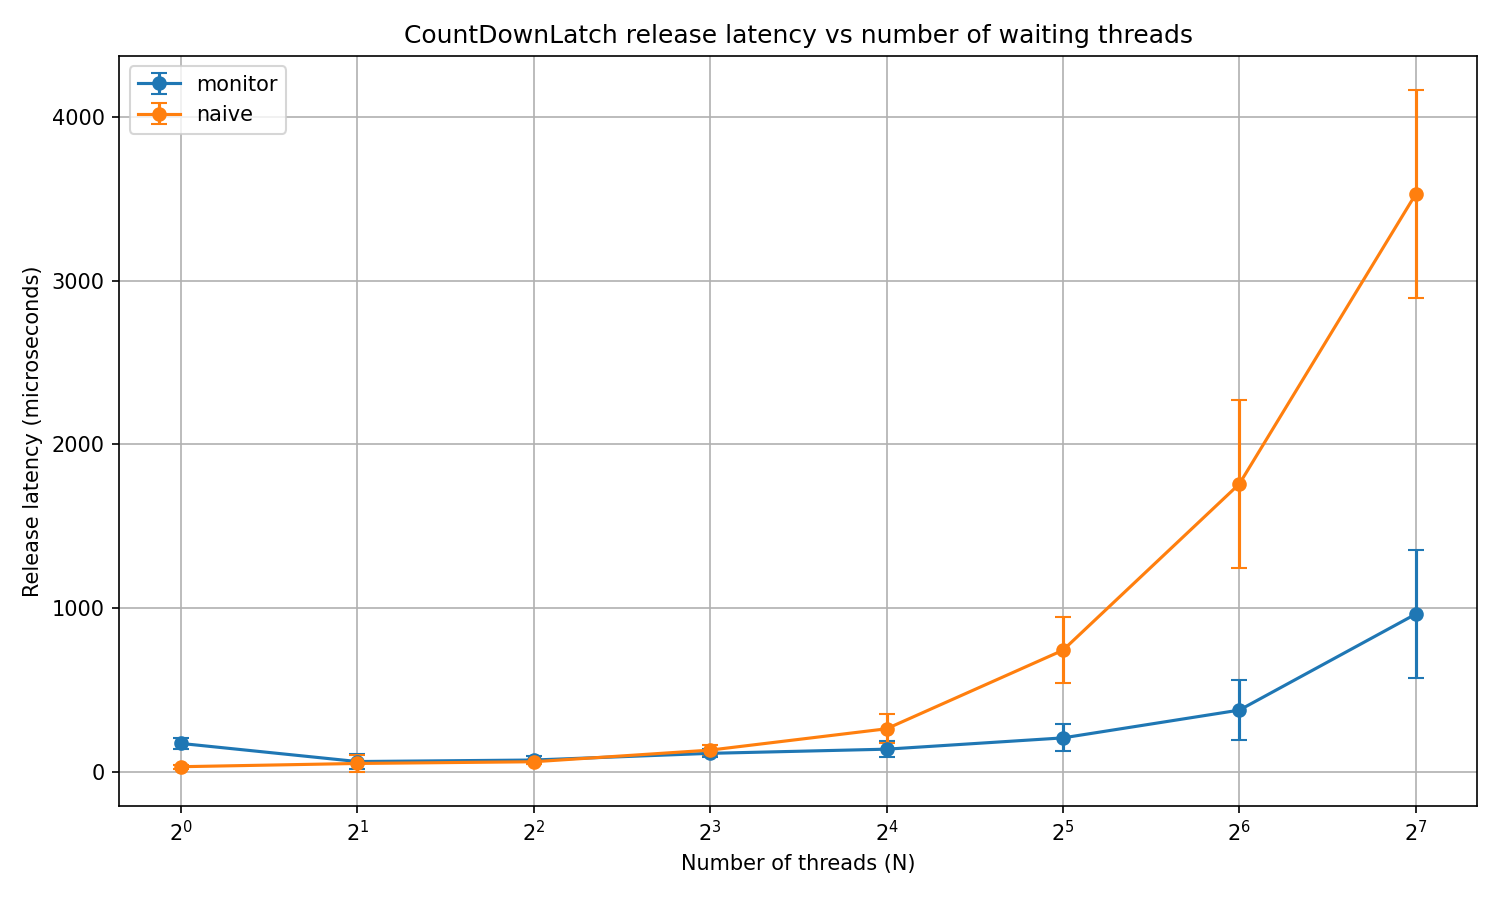
\includegraphics[width=0.9\textwidth]{../results/plot/release_latency.png}
    \caption{Release latency for NaiveCountDownLatch and MonitorCountDownLatch}
\end{figure}

\end{document}